% \usepackage{colortbl}

\chapter{Environnement professionnel et cadre de stage}
\label{ch:environnement_stage}

Dans le cadre de ma formation en Master II SIGL (Systèmes d'Information et Génie Logiciel), j'ai été amené à effectuer un stage académique au sein de l'entreprise Kairos, une structure spécialisée dans les solutions numériques et la gestion documentaire. Ce stage, d'une durée de six mois, s'est déroulé principalement au sein du département de documentation et d'archivage de l'entreprise.

Cette expérience professionnelle m'a permis d'identifier une problématique concrète liée à l'optimisation des processus métier documentaires, donnant naissance à mon projet de fin d'études intitulé : "Application de modélisation et d'automatisation des processus métier BPMN". Ce chapitre présente l'environnement professionnel dans lequel s'est déroulé mon stage, les activités de l'entreprise d'accueil, ainsi que le contexte spécifique de mon projet.

\section{Présentation de l'entreprise Kairos}

    \subsection{Historique et évolution}
    
    Kairos est une entreprise camerounaise spécialisée dans les solutions numériques et la gestion documentaire. Fondée avec pour mission de répondre aux besoins croissants des organisations en matière de digitalisation, l'entreprise s'est rapidement imposée comme un acteur de référence dans son domaine d'activité.
    
    L'entreprise a développé une expertise particulière dans l'analyse des besoins organisationnels, la proposition de solutions globales adaptées et le pilotage de leur déploiement, en respectant les contraintes de délais, de qualité et de coûts. Cette approche méthodique et centrée sur le client a contribué à la réputation de Kairos sur le marché camerounais.
    
    \subsection{Localisation et implantation}
    
    Kairos est stratégiquement implantée au Cameroun, lui permettant de servir efficacement sa clientèle locale tout en ayant une vision régionale. L'entreprise dispose d'installations modernes équipées des technologies nécessaires pour mener à bien ses missions.
    
    \begin{figure}[H]
        \center
        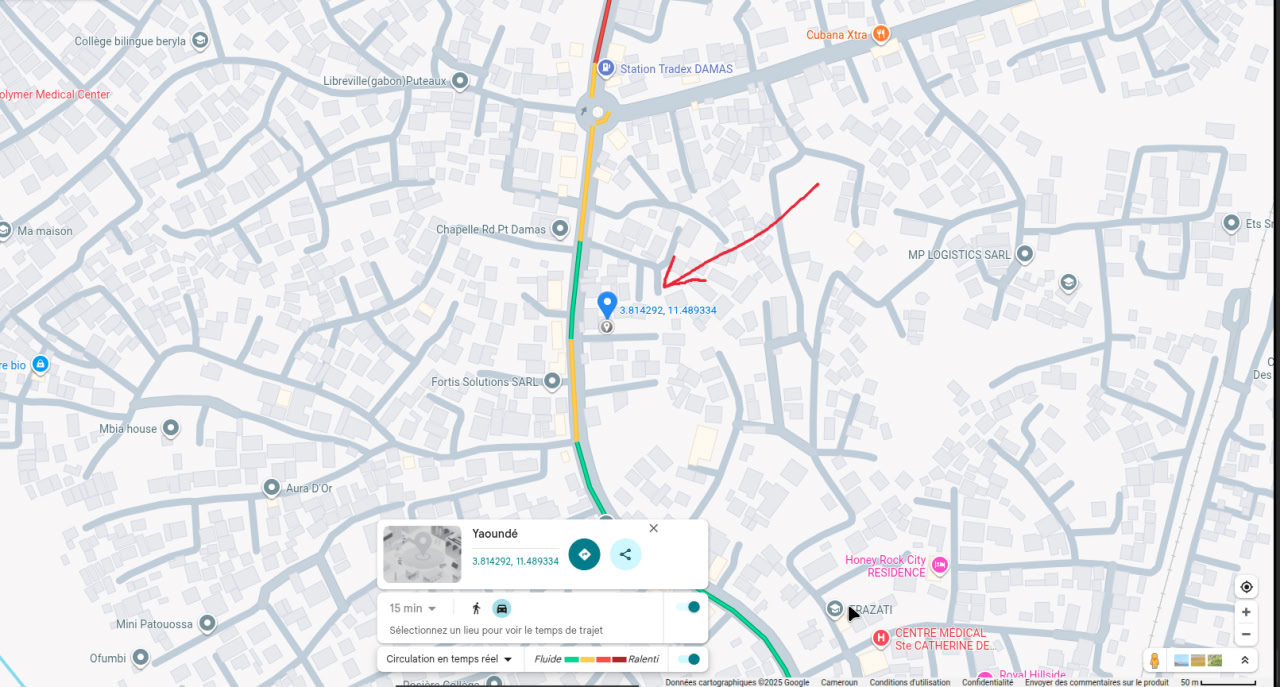
\includegraphics[width=\textwidth, height=12cm]{Images/localisation.jpg}
        \caption{Localisation GPS de KAIROS}
    \end{figure}
    
    \subsection{Mission et vision}
    
    \textbf{Mission :} Kairos analyse les besoins de ses clients, propose des solutions globales adaptées et pilote leur déploiement dans le respect des délais, de la qualité et des coûts.
    
    \textbf{Vision :} Devenir le partenaire de référence des organisations camerounaises et régionales dans leur transformation numérique et l'optimisation de leurs processus documentaires.
    
    \subsection{Domaines d'activité et services}
    
    Kairos propose une gamme complète de services structurés autour de plusieurs axes :
    
    \subsubsection{Audit et conseil}
    L'entreprise offre des prestations d'audit managérial et d'audit documentaire pour aider ses clients à atteindre leurs objectifs. Elle élabore des supports de gouvernance et fournit des conseils pour maintenir la qualité et la sécurité des données et documents.
    
    \subsubsection{Veille stratégique}
    Kairos propose des analyses et des rapports sur les informations et tendances sectorielles, permettant aux clients de prendre des décisions éclairées. L'entreprise met en place des systèmes de veille stratégique performants au sein des organisations.
    
    \subsubsection{Développement numérique}
    L'équipe de développeurs expérimentés accompagne les clients depuis le cahier des charges jusqu'à l'exploitation des solutions. Kairos propose des développements d'applications mobiles sur mesure, la création de sites web d'entreprise ergonomiques et le développement d'applications web innovantes.
    
    \subsubsection{Gestion documentaire et archivage}
    L'entreprise offre des services d'archivage physique et électronique avec des solutions sur mesure pour répondre aux besoins spécifiques de chaque client. Les services incluent également la sauvegarde et la restauration pour garantir la protection des données.
    
    \subsubsection{Formation et accompagnement}
    Kairos propose deux approches : la formation des personnels cibles dans ses métiers et l'accompagnement des équipes pour l'optimisation de leurs pratiques. Les missions incluent le renforcement des parcours professionnels, l'adaptation aux évolutions métier et l'accompagnement des changements organisationnels.
    
    \subsubsection{Gestion de projet}
    L'entreprise accompagne ses clients tout au long du cycle de projet avec une démarche d'accompagnement agile et efficace, gage de réussite pour les projets les plus complexes.
    
    \subsection{Organigramme}
    
    À la tête de l'entreprise Kairos se trouve une Directrice nommée par le conseil d'administration, choisie pour son expertise dans le domaine de la documentation et de l'archivage, sa vision stratégique et sa capacité à diriger une structure spécialisée. Elle est assistée de cinq collaborateurs directs qui pilotent l'ensemble des activités de l'entreprise.
    
    L'organisation s'articule autour d'une équipe de direction composée de :
    \begin{itemize}
        \item \textbf{Directrice} : Direction générale et vision stratégique
        \item \textbf{Attachée de direction} : Support à la direction et coordination
        \item \textbf{Responsable des opérations} : Pilotage des activités opérationnelles
        \item \textbf{Responsable commercial} : Développement commercial et relation client
        \item \textbf{Responsable administratif} : Gestion administrative et financière
        \item \textbf{Coordonnateur des services} : Coordination inter-services
    \end{itemize}
    
    Cette structure permet une organisation efficace autour de trois divisions principales : Kairos Engineering, Kairos Business et Kairos Training Center qui relèvent du Responsable des opérations. Comme le montre l'organigramme ci-dessous, l'entreprise est structurée en trois niveaux hiérarchiques clairs, avec plusieurs services spécialisés sous la supervision de chaque responsable.
    
    \vspace{1cm}
    \begin{figure}[H]
        \centering
        \centerline{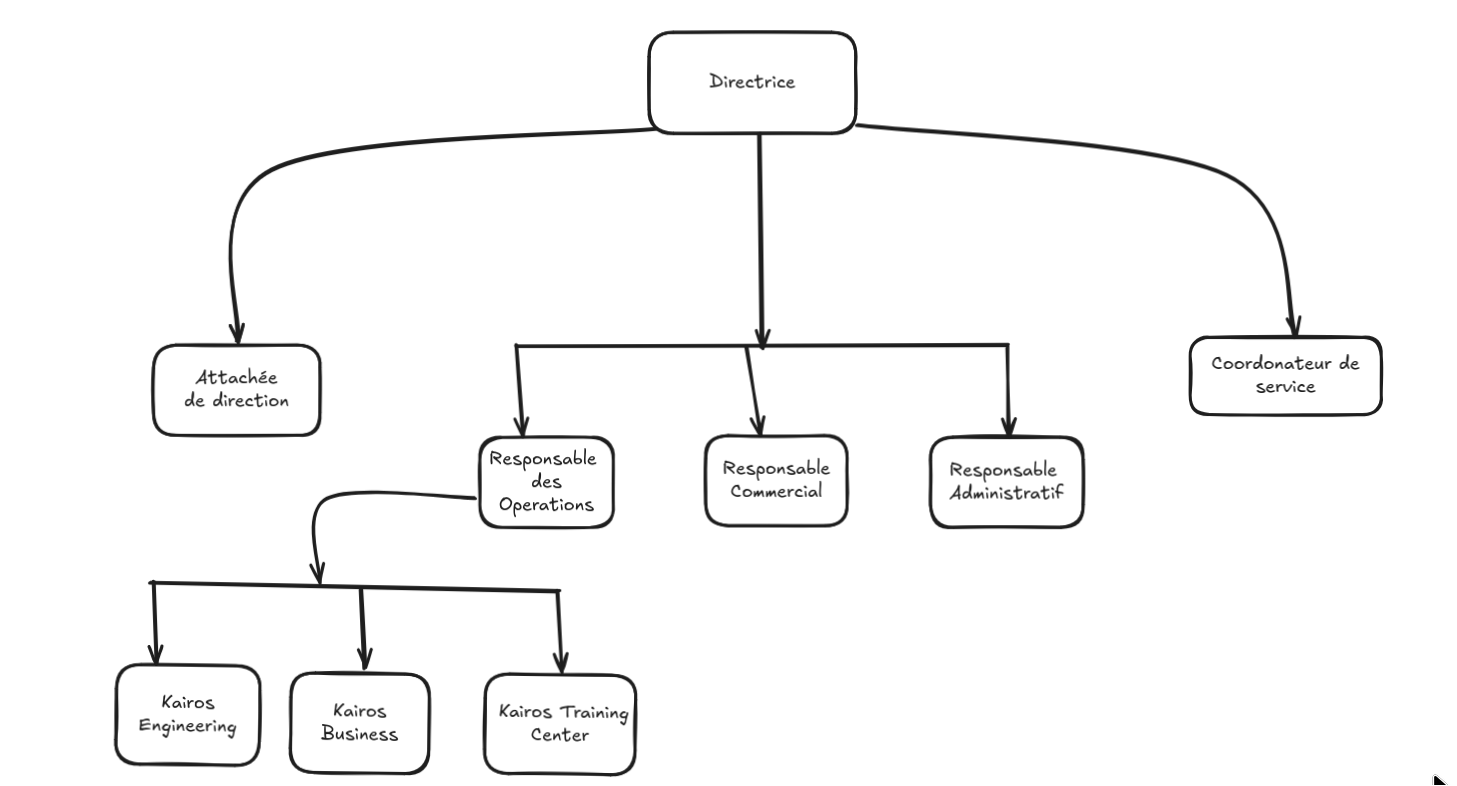
\includegraphics[width=1\linewidth]{Images/org2.png}}
        \caption{Organigramme de l'entreprise KAIROS}
        \label{fig:organigramme_kairos}
    \end{figure}

\section{Déroulement du stage et tâches effectuées}

    \subsection{Accueil et intégration}
    
    Mon intégration au sein de Kairos s'est déroulée de manière progressive et structurée. Dès les premiers jours, j'ai été présenté aux différents services et aux membres de l'équipe, permettant une compréhension globale de l'organisation et des enjeux de l'entreprise.
    
    L'accueil chaleureux et professionnel de l'équipe a facilité mon adaptation à l'environnement de travail. Un plan d'intégration avait été préparé, incluant la présentation des outils, des processus internes et des projets en cours. Cette phase d'accueil m'a également permis de mieux cerner les spécificités du département de documentation et d'archivage, lieu principal de mon stage.
    
    \subsection{Missions et tâches réalisées}
    
    Pendant le déroulement de mon stage, j'ai eu à effectuer plusieurs tâches dans le domaine de la gestion documentaire et du développement d'applications, me permettant de développer mes compétences et de contribuer concrètement aux projets de l'entreprise :
    \begin{table}[H]
        \centering
        \begin{tabularx}{\textwidth}{|l|>{\raggedright\arraybackslash}X|>{\raggedright\arraybackslash}X|}
            \hline
            \textbf{PÉRIODE} & \textbf{TACHES} & \textbf{DESCRIPTION} \\
            \hline
            Première semaine & Observation et analyse des processus & Identification des flux documentaires existants et des points d'amélioration potentiels \\
            \hline
            Deux premières semaines & Configuration de l'environnement de développement & Préparation et installation des outils et technologies nécessaires au projet BPMN \\
            \hline
            Du 15 avril au 30 juin 2024 & Implémentation de la solution BPMN & Développement de l'application \\
            % \hline
            % Tout au long du stage & Tests et validation & Vérification de la conformité de l'application aux besoins fonctionnels du projet \\
            \hline
            Fin de stage & Documentation et transfert & Rédaction de la documentation technique et formation des utilisateurs finaux \\
            \hline
        \end{tabularx}
        \caption{Déroulement détaillé du stage}
        \label{tab:deroulement_stage}
    \end{table}
    
    \subsection{Environnement technologique et apprentissages}
    
    L'environnement technique de Kairos m'a offert l'opportunité de travailler avec des technologies modernes et des outils professionnels. Le département de documentation et d'archivage utilise des solutions variées pour gérer les flux documentaires, ce qui m'a permis de mieux comprendre les enjeux de l'automatisation des processus métier.
    
    Cette expérience m'a également permis d'approfondir mes compétences en analyse de processus, en modélisation BPMN et en développement d'applications métier. La diversité des projets menés par Kairos m'a donné une vision globale des défis liés à la transformation numérique des organisations.

\section{Contexte du projet de fin d'études}

    \subsection{Problématique identifiée}
    
    Au cours de mon stage, j'ai observé que les processus documentaires de Kairos, bien qu'efficaces, présentaient des opportunités d'optimisation significatives. La gestion manuelle de certains flux de travail générait des délais de traitement et des risques d'erreur qui pouvaient être considérablement réduits grâce à une approche d'automatisation.
    
    Les principales difficultés identifiées concernent :
    \begin{itemize}
        \item La traçabilité limitée des documents dans leur cycle de vie
        \item Les redondances dans les processus de validation
        \item Les délais de traitement variables selon la charge de travail
        \item La difficulté de suivi en temps réel de l'avancement des dossiers
    \end{itemize}
    
    \subsection{Opportunité d'amélioration}
    
    L'identification de cette problématique a conduit à la définition de mon projet de fin d'études : développer une application de modélisation et d'automatisation des processus métier utilisant la notation BPMN (Business Process Model and Notation). Cette solution vise à :
    \begin{itemize}
        \item Cartographier les processus documentaires existants
        \item Identifier les goulots d'étranglement et les redondances
        \item Automatiser les tâches répétitives et chronophages
        \item Améliorer la traçabilité des documents et leur suivi
        \item Optimiser les délais de traitement global
        \item Standardiser les procédures documentaires
    \end{itemize}
    
    \subsection{Enjeux stratégiques du projet}
    
    Ce projet répond à plusieurs enjeux stratégiques majeurs pour Kairos :
    
    \textbf{Efficacité opérationnelle :} Réduction significative des temps de traitement des dossiers documentaires et optimisation de l'allocation des ressources humaines.
    
    \textbf{Qualité et fiabilité :} Minimisation des erreurs humaines grâce à l'automatisation des contrôles et des validations.
    
    \textbf{Traçabilité et conformité :} Amélioration du suivi des processus et facilitation des audits de conformité.
    
    \textbf{Évolutivité :} Mise en place d'une architecture flexible capable de s'adapter aux changements organisationnels futurs.
    
    \textbf{Compétitivité :} Positionnement de Kairos comme précurseur dans l'automatisation des processus documentaires au Cameroun.

% \section*{Conclusion}

% L'entreprise Kairos offre un environnement professionnel riche et stimulant, propice au développement de compétences techniques et managériales. La diversité de ses activités et son positionnement stratégique sur le marché de la transformation numérique en font un cadre idéal pour mener un projet d'envergure tel que celui que j'ai entrepris.

% Cette expérience de stage m'a permis de mieux comprendre les enjeux réels des entreprises en matière de gestion documentaire et d'automatisation des processus. Elle constitue le fondement solide de mon projet de fin d'études, dont les chapitres suivants détailleront les aspects techniques, méthodologiques et les résultats obtenus.

% La problématique identifiée chez Kairos illustre parfaitement les défis auxquels font face de nombreuses organisations dans leur quête d'efficacité et de digitalisation. Mon projet s'inscrit donc dans une démarche d'amélioration continue et d'innovation, valeurs chères à l'entreprise d'accueil et essentielles pour son développement futur.